\chapter{Closed Strings, Level Matching, and Duality}

\lectureoverview{A closed string supports independent waves in its two
intrinsic directions. Quantizing those waves seems at first to double the
open-string photon, but invariance under shifting the origin of the string
coordinate removes the one-sided states. The first surviving level contains
a massless spin-two particle. The same idea of changing descriptions then
opens a broader question: when couplings vary, what does it mean for any
object to be fundamental?}

\section{A Generator Kept in Reserve}

Before drawing a closed string, let us recover one fact from canonical
mechanics. Suppose
\begin{equation}
  L=L(q_i,\dot q_i),
\end{equation}
and define the momentum conjugate to \(q_i\) by
\begin{equation}
  p_i=\frac{\partial L}{\partial\dot q_i}.
\end{equation}
An infinitesimal continuous transformation can be written
\begin{equation}
  \delta q_i=\epsilon f_i(q),
  \label{eq:l04-infinitesimal-transformation}
\end{equation}
where \(\epsilon\) is a small parameter. If this transformation is a
symmetry, Noether's theorem supplies a conserved charge. Dividing the
coordinate displacement by the common parameter gives the generator
\begin{equation}
  Q=\sum_i p_i f_i(q)
   =\frac{1}{\epsilon}\sum_i p_i\,\delta q_i.
  \label{eq:l04-noether-charge}
\end{equation}
In quantum mechanics, \(Q\) is the operator that generates the corresponding
small transformation.

A rotation in the \(xy\)-plane is the familiar example. With one choice of
orientation,
\begin{equation}
  \delta x=\epsilon y,
  \qquad
  \delta y=-\epsilon x,
\end{equation}
and \eqref{eq:l04-noether-charge} becomes angular momentum, up to the same
choice of sign. The particular example will not matter. What matters is the
pattern: momentum contracted with the infinitesimal displacement gives the
generator.

\begin{figure}[H]
  \centering
  
\includegraphics[width=0.76\textwidth]{lecture_04_figure_01.png}
  \caption{The canonical momentum and Noether generator retained for the
  later shift of the closed-string coordinate.}
  \lectureframe{00:05:00}
  \label{fig:l04-noether-board}
\end{figure}

We shall shortly encounter a symmetry whose coordinate is not a point in
ordinary space but the labeling of points along a string. Equation
\eqref{eq:l04-noether-charge} is being placed within reach for that purpose.

\section{A Coordinate Around a Loop}

A closed string has no endpoints. Choose a parameter
\begin{equation}
  0\leq \sigma<2\pi
\end{equation}
and, for the moment, mark one point as \(\sigma=0\). Halfway around is
\(\sigma=\pi\); a quarter-turn and three-quarter-turn are \(\pi/2\) and
\(3\pi/2\). The mark establishes a coordinate convention, not yet a physical
feature.

\begin{figure}[H]
  \centering
  \begin{minipage}[t]{0.58\textwidth}
    \centering
    
\includegraphics[width=\textwidth]{lecture_04_figure_02.png}
    \par\smallskip\footnotesize (a) The marked loop on the blackboard.
  \end{minipage}\hfill
  \begin{minipage}[t]{0.37\textwidth}
    \centering
    \begin{adjustbox}{max width=\linewidth}
    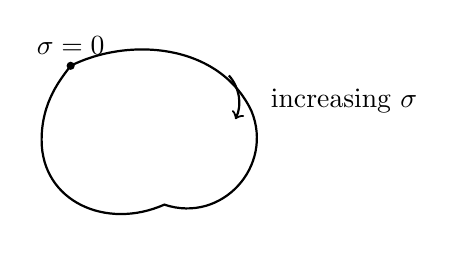
\begin{tikzpicture}[scale=0.82]
      \draw[thick]
        (0.1,1.1)
        .. controls (1.0,1.55) and (2.4,1.45) .. (2.9,0.4)
        .. controls (3.25,-0.45) and (2.45,-1.35) .. (1.55,-1.05)
        .. controls (0.65,-1.45) and (-0.35,-1.0) .. (-0.35,-0.05)
        .. controls (-0.35,0.55) and (-0.05,0.9) .. (0.1,1.1);
      \fill (0.1,1.1) circle (1.8pt);
      \node[above] at (0.1,1.12) {\(\sigma=0\)};
      \draw[->,thick] (2.55,0.95) arc[start angle=42,end angle=-25,radius=0.62];
      \node[right] at (3.05,0.55) {increasing \(\sigma\)};
    \end{tikzpicture}
    \end{adjustbox}
    \par\smallskip\footnotesize (b) The intrinsic orientation.
  \end{minipage}
  \caption{A point is marked to define the origin, and an arrow fixes the
  direction in which \(\sigma\) increases.}
  \lectureframe{00:06:48}
  \label{fig:l04-closed-string-origin}
\end{figure}

The arrow along the loop is an \emph{intrinsic} orientation. It must not be
confused with clockwise or counterclockwise motion in the \(xy\)-plane.
Imagine a marked rubber band lifted from the board, turned over, and put back.
Its apparent clockwise sense reverses, while the sequence of its intrinsic
marks does not. Increasing \(\sigma\) remains increasing \(\sigma\).

This distinction controls the language of right- and left-moving waves. In
this chapter, a right-moving disturbance means one traveling toward
increasing \(\sigma\), and a left-moving disturbance means one traveling
toward decreasing \(\sigma\). Neither name tells us which way the disturbance
appears to move in the room.

Orientation had a concrete role in the original hadronic string picture.
Breaking an oriented flux tube produces a quark at one endpoint and an
antiquark at the other; the intrinsic arrow distinguishes the two ends. One
can also construct unoriented string theories, but for the present discussion
we retain the arrow and the two senses along it.

\section{Periodicity and Running Waves}

Let \(X(\sigma,\tau)\) and \(Y(\sigma,\tau)\) be two transverse coordinates of
the string, with \(\tau\) denoting time. Extra transverse coordinates, when
present, are treated in exactly the same way. Since \(\sigma=0\) and
\(\sigma=2\pi\) label the same point,
\begin{equation}
  X(\sigma+2\pi,\tau)=X(\sigma,\tau),
  \qquad
  Y(\sigma+2\pi,\tau)=Y(\sigma,\tau).
  \label{eq:l04-periodicity}
\end{equation}

\begin{figure}[H]
  \centering
  
\includegraphics[width=0.76\textwidth]{lecture_04_figure_03.png}
  \caption{Periodic boundary conditions for the two transverse coordinates.}
  \lectureframe{00:12:40}
  \label{fig:l04-periodicity-board}
\end{figure}

A localized wiggle can therefore circulate indefinitely. When it reaches
\(2\pi\), it simply reappears at \(0\). This differs from an open string,
where a running wave reaches an endpoint and reflects; what was left-moving
becomes right-moving and vice versa. Standing waves are natural for the open
string, whereas a closed string admits two independently propagating
families.

\subsection{Complex Fourier modes}

The convenient basis for a periodic function is
\begin{equation}
  e^{in\sigma}=\cos(n\sigma)+i\sin(n\sigma),
  \qquad n\in\mathbb Z.
\end{equation}
The integer condition is forced by periodicity:
\(e^{in(\sigma+2\pi)}=e^{in\sigma}\). Replacing \(n\) by a half-integer, for
example, would change the function after one circuit.

Suppressing time dependence momentarily, the blackboard expansion is
\begin{align}
  X(\sigma)
  &=
  X_0+
  \sum_{n>0}X_n e^{in\sigma}
  +\sum_{n>0}X_{-n}e^{-in\sigma},
  \label{eq:l04-fourier-x}\\
  Y(\sigma)
  &=
  Y_0+
  \sum_{n>0}Y_n e^{in\sigma}
  +\sum_{n>0}Y_{-n}e^{-in\sigma}.
  \label{eq:l04-fourier-y}
\end{align}
For real \(X\) and \(Y\), the negative-index coefficients are complex
conjugates of the positive-index coefficients at the classical level. The
zero modes \(X_0\) and \(Y_0\) locate the center of mass; they are positions,
not internal oscillations.

\begin{figure}[H]
  \centering
  
\includegraphics[width=0.82\textwidth]{lecture_04_figure_04.png}
  \caption{The positive- and negative-index pieces of the periodic Fourier
  expansion, followed by the zero mode.}
  \lectureframe{00:20:00}
  \label{fig:l04-fourier-board}
\end{figure}

\begin{classroomqa}
\audiencequestion{If these are moving waves, where is the time
coordinate?\lecturetimestamp{00:19:05}}
\lecturerresponse{It has only been suppressed in the board notation. A
traveling solution carries a phase involving both \(\sigma\) and \(\tau\).
With the convention used below, one family has
\(e^{-in(\tau-\sigma)}\) and the other
\(e^{-in(\tau+\sigma)}\).}
\end{classroomqa}

Thus it is the full phase, not the sign of \(n\) in a purely spatial Fourier
factor by itself, that determines propagation. We may write
\begin{equation}
  X(\sigma,\tau)=X_R(\tau-\sigma)+X_L(\tau+\sigma),
  \label{eq:l04-chiral-solution}
\end{equation}
and similarly for \(Y\). Which family is called \(R\) rather than \(L\) is a
convention; the invariant fact is that there are two opposite directions
along the \(\sigma\)-circle.\editorialnote{A factor \(e^{in\sigma}\) at one
instant does not by itself specify a moving wave. Propagation is fixed only
after the time phase is supplied.}

\section{Energy in the Two Directions}

The local dynamics is the same as for the open string. In the simplified
normalization used here,
\begin{equation}
  L\propto
  \int_0^{2\pi}d\sigma\,
  \left[
    \dot X^2-X'^2+\dot Y^2-Y'^2
  \right],
  \label{eq:l04-string-lagrangian}
\end{equation}
where a dot denotes \(\partial_\tau\) and a prime denotes
\(\partial_\sigma\). The energy has a plus sign between kinetic and elastic
terms:
\begin{equation}
  E\propto
  \int_0^{2\pi}d\sigma\,
  \left[
    \dot X^2+X'^2+\dot Y^2+Y'^2
  \right].
  \label{eq:l04-string-energy}
\end{equation}
For either transverse coordinate,
\begin{equation}
  \dot X^2+X'^2
  =
  \frac12(\dot X+X')^2+
  \frac12(\dot X-X')^2.
  \label{eq:l04-energy-square-completion}
\end{equation}
The cross terms cancel, leaving precisely the original kinetic and gradient
energies.

\begin{figure}[H]
  \centering
  
\includegraphics[width=0.82\textwidth]{lecture_04_figure_05.png}
  \caption{The total energy reorganized into the two running-wave sectors.}
  \lectureframe{00:25:10}
  \label{fig:l04-energy-board}
\end{figure}

For \(X_R(\tau-\sigma)\), one has \(\dot X_R=-X_R'\); for
\(X_L(\tau+\sigma)\), one has \(\dot X_L=X_L'\). Consequently the two
squares in \eqref{eq:l04-energy-square-completion} isolate the two chiral
families. Including every transverse coordinate, define
\begin{align}
  E_L&\propto
  \frac12\int_0^{2\pi}d\sigma
  \sum_I(\dot X^I+X^{I\prime})^2,\\
  E_R&\propto
  \frac12\int_0^{2\pi}d\sigma
  \sum_I(\dot X^I-X^{I\prime})^2.
  \label{eq:l04-left-right-energies}
\end{align}
Then \(E=E_L+E_R\). Because the equations are linear at this stage, waves
from the two sectors pass through one another without scattering.

\subsection{Twice as many oscillators}

Substituting the Fourier series into
\eqref{eq:l04-string-lagrangian} turns each nonzero mode coefficient into a
harmonic oscillator. Its frequency is proportional to \(|n|\): shorter
wavelength means higher frequency and therefore a larger excitation energy.
Unlike the open string, each positive frequency occurs in two independently
propagating copies.

The blackboard labels the \(X\)-polarized creation operators
\(a_n^+\) and \(a_{-n}^+\), and the \(Y\)-polarized ones
\(b_n^+\) and \(b_{-n}^+\). To separate creation from propagation more
cleanly, we shall write
\begin{equation}
  a_n^\dagger,\quad b_n^\dagger,
  \qquad
  \widetilde a_n^\dagger,\quad\widetilde b_n^\dagger,
  \qquad n>0.
  \label{eq:l04-oscillator-notation}
\end{equation}
The untilded and tilded operators create opposite world-sheet directions;
\(a\) and \(b\) denote the two transverse polarizations.

\begin{figure}[H]
  \centering
  
\includegraphics[width=0.65\textwidth]{lecture_04_figure_06.png}
  \caption{The board notation for the doubled \(X\)- and \(Y\)-polarized
  creation operators.}
  \lectureframe{00:29:10}
  \label{fig:l04-oscillators-board}
\end{figure}

If \(N_n^{(a)},N_n^{(b)}\) and their tilded partners are occupation numbers,
the oscillator levels carried in the two directions are schematically
\begin{equation}
  \begin{aligned}
    N&=\sum_{n>0}n\bigl(N_n^{(a)}+N_n^{(b)}+\cdots\bigr),\\
    \widetilde N&=\sum_{n>0}n
      \bigl(\widetilde N_n^{(a)}+\widetilde N_n^{(b)}+\cdots\bigr).
  \end{aligned}
  \label{eq:l04-level-operators}
\end{equation}
The ellipses stand for additional transverse directions.

\section{The Spectrum Guess That Fails}

Recall the open-string first level. Acting on the ground state with
\(a_1^\dagger\) or \(b_1^\dagger\) gives two linear polarizations. Their
circular combinations,
\begin{equation}
  c_\pm^\dagger
  =
  \frac{1}{\sqrt2}
  \left(a_1^\dagger\pm i b_1^\dagger\right),
  \label{eq:l04-open-circular}
\end{equation}
carry helicity \(h=\pm1\). The absence of a helicity-zero partner is the
signature of a massless vector in this elementary four-dimensional
description.

Let the closed-string ground state have mass squared \(m_0^2\). A first,
naive guess is to act once with any one of
\begin{equation}
  a_1^\dagger,\quad b_1^\dagger,\quad
  \widetilde a_1^\dagger,\quad\widetilde b_1^\dagger.
  \label{eq:l04-naive-one-sided}
\end{equation}
This resembles two copies of the open-string photon, one for each propagation
direction. At the next energy, however, the unrestricted list does not
assemble into sensible rotational multiplets. The problem is not repaired by
more elaborate bookkeeping. The premise that every oscillator monomial is a
physical state is wrong.

\subsection{Level matching, first as a rule}

The physical closed-string condition is
\begin{equation}
  N=\widetilde N,
  \qquad\text{equivalently}\qquad E_L=E_R.
  \label{eq:l04-level-matching}
\end{equation}
For the moment, take this as a postulate; its origin will be derived only
after we have seen what it accomplishes.

Every state in \eqref{eq:l04-naive-one-sided} has one unit of energy in one
sector and none in the other, so every one is excluded. The first surviving
states carry one oscillator from each family:
\begin{align}
  a_1^\dagger\widetilde a_1^\dagger\ket{0},
  &\qquad
  b_1^\dagger\widetilde b_1^\dagger\ket{0},
  \label{eq:l04-four-matched-a}\\
  a_1^\dagger\widetilde b_1^\dagger\ket{0},
  &\qquad
  b_1^\dagger\widetilde a_1^\dagger\ket{0}.
  \label{eq:l04-four-matched-b}
\end{align}
They have total oscillator energy two, divided equally between the two
directions. A single \(n=2\) creation operator has the same total oscillator
energy but fails \eqref{eq:l04-level-matching}; it contributes two units to
only one side.

\begin{figure}[H]
  \centering
  
\includegraphics[width=0.70\textwidth]{lecture_04_figure_07.png}
  \caption{The four first-level states that survive level matching. The board
  uses subscripts \(1\) and \(-1\) where
  \eqref{eq:l04-four-matched-a}--\eqref{eq:l04-four-matched-b} use untilded
  and tilded operators.}
  \lectureframe{00:41:05}
  \label{fig:l04-level-matched-board}
\end{figure}

\section{A Graviton in the First Matched Level}

Put both chiral families into a circular basis:
\begin{equation}
  c_\pm^\dagger
  =\frac{a_1^\dagger\pm i b_1^\dagger}{\sqrt2},
  \qquad
  \widetilde c_\pm^\dagger
  =\frac{\widetilde a_1^\dagger\pm i\widetilde b_1^\dagger}{\sqrt2}.
  \label{eq:l04-closed-circular}
\end{equation}
Each factor contributes helicity \(+1\) or \(-1\) in ordinary transverse
space. Their products therefore give
\begin{center}
\begin{tabular}{c c}
  \toprule
  State & Helicity \\
  \midrule
  \(c_+^\dagger\widetilde c_+^\dagger\ket0\) & \(+2\) \\
  \(c_-^\dagger\widetilde c_-^\dagger\ket0\) & \(-2\) \\
  \(c_+^\dagger\widetilde c_-^\dagger\ket0\) & \(0\) \\
  \(c_-^\dagger\widetilde c_+^\dagger\ket0\) & \(0\) \\
  \bottomrule
\end{tabular}
\end{center}

\begin{classroomqa}
\audiencequestion{Should the second circular-polarization factor come from
the opposite propagation sector?\lecturetimestamp{00:43:20}}
\lecturerresponse{Yes. The first expression written on the board was
corrected for precisely this reason. A physical state here must pair one
right-moving oscillator with one left-moving oscillator; otherwise it is not
level matched. The helicities refer to transverse-space polarization, while
the two factors refer to opposite world-sheet directions.}
\end{classroomqa}

\begin{figure}[H]
  \centering
  
\includegraphics[width=0.82\textwidth]{lecture_04_figure_08.png}
  \caption{The four circular-basis products after the board correction, with
  helicities \(+2,-2,0,0\).}
  \lectureframe{00:46:10}
  \label{fig:l04-helicity-board}
\end{figure}

A massive spin-two particle has five spin projections,
\begin{equation}
  m=2,1,0,-1,-2.
\end{equation}
The matched level contains no \(m=\pm1\) partners. It therefore cannot be a
massive spin-two multiplet. A massless spin-two particle, by contrast, has
only helicities \(+2\) and \(-2\). The same-helicity products are exactly
those two states: they are the graviton polarizations.

Two helicity-zero combinations remain. In the language used in class, one is
the dilaton and the other the axion. A covariant description of the generic
closed bosonic string refines this statement:
\begin{equation}
  \begin{aligned}
    \alpha_{-1}^{I}\widetilde\alpha_{-1}^{J}\ket{0;k}
    &\longrightarrow
    \underbrace{h_{IJ}}_{\text{symmetric traceless}}
    \oplus
    \underbrace{B_{IJ}}_{\text{antisymmetric}}\\
    &\hspace{2.5em}\oplus
    \underbrace{\Phi}_{\text{trace}}.
  \end{aligned}
  \label{eq:l04-massless-tensor-decomposition}
\end{equation}
These are the graviton, antisymmetric two-form, and dilaton. In four
dimensions the two-form can be dualized to an axion-like pseudoscalar, which
is the language adopted in the lecture.\editorialnote{The second
helicity-zero state is fundamentally the antisymmetric tensor field
\(B_{\mu\nu}\) in the generic closed-string spectrum. Calling it an axion is
the four-dimensional dual description.}

At this formal level the three fields are massless. Compactification,
projections, and background dynamics can alter which scalar or two-form
degrees of freedom remain light. The graviton is different: once a
consistent interacting closed-string sector is present, its massless
spin-two state is unavoidable. This is why gravity emerges from closed
strings rather than being appended as a separate ingredient.

\section{Why the Levels Must Match}

We now return to the mark at \(\sigma=0\). Is it a physical bead attached to
the loop, or merely the origin of our parameter? For an ordinary unmarked
closed string, no point should be privileged. The quantum state must be
unchanged when every label is shifted together.

\subsection{The discrete version}

Regulate the loop as \(M\) ordered points with transverse coordinates
\((X_i,Y_i)\). Temporarily suppress \(Y_i\). A configuration-space
wavefunction is
\begin{equation}
  \Psi(X_1,X_2,\ldots,X_M).
\end{equation}
Changing which point is called first gives a cyclic permutation:
\begin{align}
  \Psi(X_1,X_2,\ldots,X_M)
  &=
  \Psi(X_2,\ldots,X_M,X_1)\nonumber\\
  &=
  \Psi(X_3,\ldots,X_M,X_1,X_2).
  \label{eq:l04-cyclic-wavefunction}
\end{align}
This is not invariance under an arbitrary permutation. Inserting \(X_3\)
between \(X_1\) and \(X_2\), for example, changes the adjacency structure and
effectively tears and reconnects the discretized string. Only the common
cyclic relabeling
\begin{equation}
  X_i\longrightarrow X_{i+1}\qquad(\text{mod }M)
  \label{eq:l04-discrete-shift}
\end{equation}
expresses the absence of a preferred origin.

\begin{figure}[H]
  \centering
  
\includegraphics[width=0.82\textwidth]{lecture_04_figure_09.png}
  \caption{The cyclic wavefunction identities for a discretized closed
  string.}
  \lectureframe{00:56:20}
  \label{fig:l04-cyclic-board}
\end{figure}

\subsection{The continuum version}

As \(M\to\infty\), the state becomes a wavefunctional
\(\Psi[X(\sigma),Y(\sigma)]\), and the cyclic relabeling becomes
\begin{equation}
  \sigma\longrightarrow\sigma+\epsilon.
\end{equation}
Invariance says
\begin{equation}
  \Psi[X(\sigma+\epsilon),Y(\sigma+\epsilon)]
  =
  \Psi[X(\sigma),Y(\sigma)].
  \label{eq:l04-wavefunctional-invariance}
\end{equation}

\begin{figure}[H]
  \centering
  
\includegraphics[width=0.72\textwidth]{lecture_04_figure_10.png}
  \caption{The discrete shift and its wavefunctional continuum form.}
  \lectureframe{00:58:40}
  \label{fig:l04-wavefunctional-board}
\end{figure}

To first order,
\begin{equation}
  \delta X(\sigma)=\epsilon X'(\sigma),
  \qquad
  \delta Y(\sigma)=\epsilon Y'(\sigma),
  \label{eq:l04-profile-shift}
\end{equation}
up to the overall sign that distinguishes an active shift of the profile from
a passive shift of the coordinate. The corresponding wavefunctional
variation is
\begin{equation}
  \delta\Psi
  =
  \epsilon\int_0^{2\pi}d\sigma
  \left[
    \frac{\delta\Psi}{\delta X(\sigma)}X'(\sigma)
    +
    \frac{\delta\Psi}{\delta Y(\sigma)}Y'(\sigma)
  \right].
  \label{eq:l04-functional-variation}
\end{equation}

\begin{figure}[H]
  \centering
  
\includegraphics[width=0.72\textwidth]{lecture_04_figure_11.png}
  \caption{The first-order expansion of the shifted wavefunctional
  argument.}
  \lectureframe{01:01:31}
  \label{fig:l04-functional-expansion-board}
\end{figure}

\begin{classroomqa}
\audiencequestion{Is the first-order condition a separate equation for each
value of \(\sigma\)?\lecturetimestamp{01:01:30}}
\lecturerresponse{No. The transformation shifts every point of the string
together. The variation at one point must be added to the variations at all
other points, which is why the continuum expression contains the integral
over \(\sigma\).}
\end{classroomqa}

In the coordinate representation,
\begin{equation}
  P_X(\sigma)=-i\frac{\delta}{\delta X(\sigma)},
  \qquad
  P_Y(\sigma)=-i\frac{\delta}{\delta Y(\sigma)}
  \label{eq:l04-functional-momenta}
\end{equation}
with \(\hbar=1\). Equation \eqref{eq:l04-functional-variation} is therefore
generated by
\begin{equation}
  G_\sigma=
  \int_0^{2\pi}d\sigma\,
  \left[
    P_X(\sigma)X'(\sigma)+P_Y(\sigma)Y'(\sigma)
  \right].
  \label{eq:l04-sigma-generator}
\end{equation}
This is exactly the Noether pattern
\eqref{eq:l04-noether-charge}: canonical momentum multiplied by the
coordinate displacement, summed over all degrees of freedom. An unmarked
closed-string state obeys
\begin{equation}
  G_\sigma\ket{\mathrm{phys}}=0.
  \label{eq:l04-physical-generator-condition}
\end{equation}

For the normalization of \eqref{eq:l04-string-lagrangian},
\(P_I\propto\dot X^I\), so the same condition reads
\begin{equation}
  \int_0^{2\pi}d\sigma
  \sum_I\dot X^I X^{I\prime}=0.
  \label{eq:l04-momentum-constraint}
\end{equation}

\begin{figure}[H]
  \centering
  
\includegraphics[width=0.75\textwidth]{lecture_04_figure_12.png}
  \caption{The integrated generator after the derivative of the
  wavefunctional is identified with momentum.}
  \lectureframe{01:05:10}
  \label{fig:l04-generator-board}
\end{figure}

\subsection{The generator is the energy difference}

The sum of the two expressions in
\eqref{eq:l04-left-right-energies} is the total energy. Their difference is
\begin{align}
  E_L-E_R
  &\propto
  \frac12\int_0^{2\pi}d\sigma\sum_I
  \left[
    (\dot X^I+X^{I\prime})^2\right.\nonumber\\[-0.25em]
  &\hspace{7em}\left.
    -(\dot X^I-X^{I\prime})^2
  \right]\\
  &=
  2\int_0^{2\pi}d\sigma\sum_I
  \dot X^I X^{I\prime}.
  \label{eq:l04-energy-difference}
\end{align}
The integral is the generator that must annihilate a physical state.
Therefore
\begin{equation}
  E_L-E_R=0,
  \qquad\text{or}\qquad
  N-\widetilde N=0.
\end{equation}
Level matching is the statement that the origin of the \(\sigma\)-coordinate
is unobservable.

\begin{figure}[H]
  \centering
  
\includegraphics[width=0.78\textwidth]{lecture_04_figure_13.png}
  \caption{The energy sum and difference displayed together at the end of
  the level-matching derivation.}
  \lectureframe{01:06:40}
  \label{fig:l04-energy-difference-board}
\end{figure}

\begin{classroomqa}
\audiencequestion{Why do the displayed formulas appear to place the factor
of one-half differently?\lecturetimestamp{01:06:28}}
\lecturerresponse{Only the relative structure is being used. Restoring one
consistent overall normalization gives the one-half in the completed-square
identity \eqref{eq:l04-energy-square-completion}. The sum yields total energy,
while the difference remains proportional to
\(\int d\sigma\,\dot X X'\). Its vanishing, and hence level matching, is
independent of that common convention.}
\end{classroomqa}

The constraint removes a large portion of the naive oscillator spectrum, and
it removes precisely the states that failed to form sensible particle
multiplets. It does not remove the open-string photon, because an open string
does not possess two independent circulating sectors subject to this closed
loop condition. For the closed string, it leaves the graviton, the dilaton,
the antisymmetric-tensor or axion-like state, and the higher matched levels.
\editorialnote{In covariant string quantization, level matching is the
zero-mode condition \(L_0-\widetilde L_0=0\), one member of the world-sheet
constraint system. The derivation here isolates its intuitive origin as
invariance under translations around the closed string.}

\section{Two Meanings of Left and Right}

There are now two unrelated uses of handed language:
\begin{enumerate}
  \item \(X_R(\tau-\sigma)\) and \(X_L(\tau+\sigma)\) describe propagation
  toward opposite directions along the intrinsic \(\sigma\)-circle.
  \item \(c_+^\dagger\) and \(c_-^\dagger\) describe circular polarization in
  the physical transverse \(xy\)-plane.
\end{enumerate}
The level-matched graviton state contains one oscillator from each
world-sheet direction. Those two oscillators may nevertheless have the same
spacetime helicity, producing \(h=+2\) or \(h=-2\). Confusing these two kinds
of left and right makes the spectrum look contradictory when it is not.

\section{What Does Fundamental Mean?}

Once open and closed strings have been quantized at this elementary level, a
natural question remains: are strings the final constituents, or could they
themselves be made of something else?

\begin{classroomqa}
\audiencequestion{Is there evidence or a reason to regard strings as the most
fundamental objects, with nothing smaller underneath
them?\lecturetimestamp{01:10:44}}
\lecturerresponse{There is no useful parameter-independent answer. The
degrees of freedom that look elementary in one regime can become heavy,
extended, and apparently composite in another. Fundamental is best read as a
statement about which variables provide the useful description at the
coupling under consideration.}
\end{classroomqa}

Electric and magnetic charges provide the cleanest model of this answer.
Suppose a theory contains an electric charge \(e\) and a magnetic charge
\(g\). The unobservable Dirac string attached to a monopole requires
\begin{equation}
  eg=2\pi n,
  \qquad n\in\mathbb Z.
  \label{eq:l04-dirac-quantization}
\end{equation}
For the minimal charges, \(n=1\). A charged particle circling the Dirac
string then acquires a phase \(e^{ieg}=1\), so the auxiliary string cannot be
detected.

\begin{figure}[H]
  \centering
  \begin{minipage}[t]{0.58\textwidth}
    \centering
    
\includegraphics[width=\textwidth]{lecture_04_figure_14.png}
    \par\smallskip\footnotesize (a) Dirac quantization on the board.
  \end{minipage}\hfill
  \begin{minipage}[t]{0.36\textwidth}
    \centering
    \begin{adjustbox}{max width=\linewidth}
    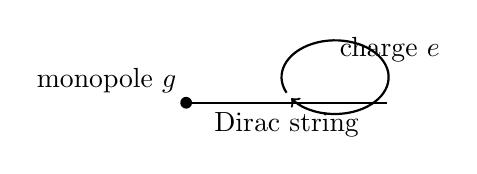
\begin{tikzpicture}[scale=0.85]
      \fill (0,0) circle (2.5pt);
      \node[above left] at (0,0) {monopole \(g\)};
      \draw[thick] (0,0) -- (3.0,0);
      \node[below] at (1.5,0) {Dirac string};
      \draw[->,thick] (1.5,0.15) arc[start angle=205,end angle=-145,
        x radius=0.8,y radius=0.55];
      \node[right] at (2.15,0.8) {charge \(e\)};
    \end{tikzpicture}
    \end{adjustbox}
    \par\smallskip\footnotesize (b) The phase experiment around the string.
  \end{minipage}
  \caption{Electric and magnetic charges are inversely related by the Dirac
  condition.}
  \lectureframe{01:13:20}
  \label{fig:l04-dirac-board}
\end{figure}

If \(e\) is small, ordinary perturbation theory in electric variables is
useful. Feynman diagrams with additional electric vertices are increasingly
suppressed. But \eqref{eq:l04-dirac-quantization} then makes \(g\) large, so a
diagrammatic expansion in magnetic vertices is not useful. In terms of the
usual dimensionless couplings,
\begin{equation}
  \alpha_e=\frac{e^2}{4\pi},
  \qquad
  \alpha_m=\frac{g^2}{4\pi},
  \qquad
  \alpha_e\alpha_m=\frac{n^2}{4}.
  \label{eq:l04-dual-couplings}
\end{equation}
Weak electric coupling is strong magnetic coupling, and conversely.

The strongly coupled monopole also looks complicated from the electric
description. Its field energy is large; it is dressed by an intense cloud of
gauge-field fluctuations and virtual magnetically charged pairs. It behaves
as a heavy, extended object, a poor starting point for an electric
perturbation series. This does not prove that it is less fundamental. It says
that it is the wrong elementary variable for that regime.

Now imagine continuously increasing \(e\). The quantization condition forces
\(g\) to decrease. Near the self-dual region neither description is
especially weak, and beyond it the magnetic variables can become the simpler,
lighter ones while the electric objects become strongly dressed. Which
charge should be called elementary has changed without changing the theory's
physical content.

\subsection{The Wigner question}

This ambiguity once surfaced in a discussion of whether the Higgs boson was
fundamental or composite. Eugene Wigner repeatedly asked what composite
meant. One proposed distinction was decay: perhaps a fundamental object
cannot decay and a composite object can. But a ground-state hydrogen atom
cannot decay and is plainly composite; the proton may be stable while the
neutron decays, yet that does not make one elementary and the other composite
in the intended sense. Every simple definition generated another
counterexample.

Gerardus 't Hooft ended the discussion with the operational criterion: an
object is fundamental when it is useful to think of it as fundamental. This
is not an evasion. It recognizes that elementary identifies the variables in
which the dynamics is simple, and simplicity can depend on coupling and
environment.

\section{Toward M-Theory}

String theory realizes this exchange of roles in a particularly sharp way.
In one parameter regime, strings are light and perturbative, while D-branes
look like heavy solitonic composites built from string degrees of freedom. As
the parameters change, D-branes can become the lighter elementary objects,
and configurations described as strings in the first regime can be
reinterpreted in terms of them. What looked fundamental can become composite;
what looked composite can become fundamental.

The old reductionist picture suggests a one-way descent from large things to
smaller constituents and finally to a unique bottom layer. Duality suggests
something less linear: descriptions can transform into one another as
couplings vary, with no single set of variables privileged everywhere. That
is the angle from which the next subject, M-theory, will be approached.

The questions of why the critical dimensions are twenty-six for the bosonic
string and ten for the superstring remain open here. Rather than settling
every technical issue before moving on, we now change viewpoint and ask how
M-theory can produce string theory in an appropriate limit.
